\section{Parallel Huffman implementation}
To parallelize the serial Huffman algorithm over threads and processes, we decided to follow this simple yet effective structure:
\begin{itemize}
    \item Multiple processes should handle groups of file and folders separately.
    \item Multiple threads of the same process should work on different chunks of the same file in parallel.
\end{itemize}
Specifically, there are multiple reasons behind our parallel architectural design for this project. Here follows a list of the main ones:
\begin{itemize}
	\item In most operating systems a file is a resource that the OS gives to a single process to avoid race conditions. We wanted to follow a similar design philosophy.
	\item Most operating systems allow multiple processes to open the same file in reading mode, but only few allow to open the same file in writing mode on multiple processes. This is because that leads to potentially concurrency and data integrity issues. By ensuring to have only a single process that open a specific file, we avoid all these issues.
	\item Because threads of the same process share the address space, we can avoid the expensive data transfer across processes. When data is read or written to file, there is no need to transfer data between threads.
\end{itemize}
In the next section, we start by explaining the basic multithreading operations on a single file. Later on, multiprocessing with multiple files is covered.

\subsection{Multithreading}

The parallel algorithm for a single file follows the exact same procedure as for the serial version, with just a few key differences to allow multithreading. 

Suppose we are dealing with \(m\) threads and a single input file. Here follows a common procedure used for both encoding and decoding, with very small differences. 
\begin{enumerate}
	\item A single file is divided into chunks of a fixed size. When that is done, the single process forks and creates \(m\) threads.
	\item A single thread (may be the main one, may not ) then reads \(m\) chunks in a shared memory buffer.
	\item Each one of the \(m\) threads works in parallel on the processing of its assigned chunk using a buffer. Although all the chunks are in shared memory buffer, each thread is assigned only to a single memory section: in this way there is no need to care about racing conditions when writing in the buffer. This is done by creating a \verb|unsigned char buffer[m][buffer_size]|. 
	\item When all threads are done computing, either the encoding or decoding of their chunks, a single thread writes the processed chunks to the output file.
	Again, since all threads share a memory space there is no need to perform data transfer.
\end{enumerate}

Moreover, our implementation also parallelize the counting of occurrences of a byte in the input file, since this is required in order to create the Huffman tree. 
This is done only during the encoding phase, as for the decoding the occurences are no longer required because the huffman tree is already saved in the encoded data. The procedure is very similar to the one just described, with the key difference that there is no output file to write, but only byte occurrences stored in an in-memory array unique for each thread to avoid concurrency. When the counting is done, all threads join their counts into a single array.

 \Cref{fig:threading} shows a schema of the parallel workflow for processing a single file. 

\begin{figure}
	\centering
	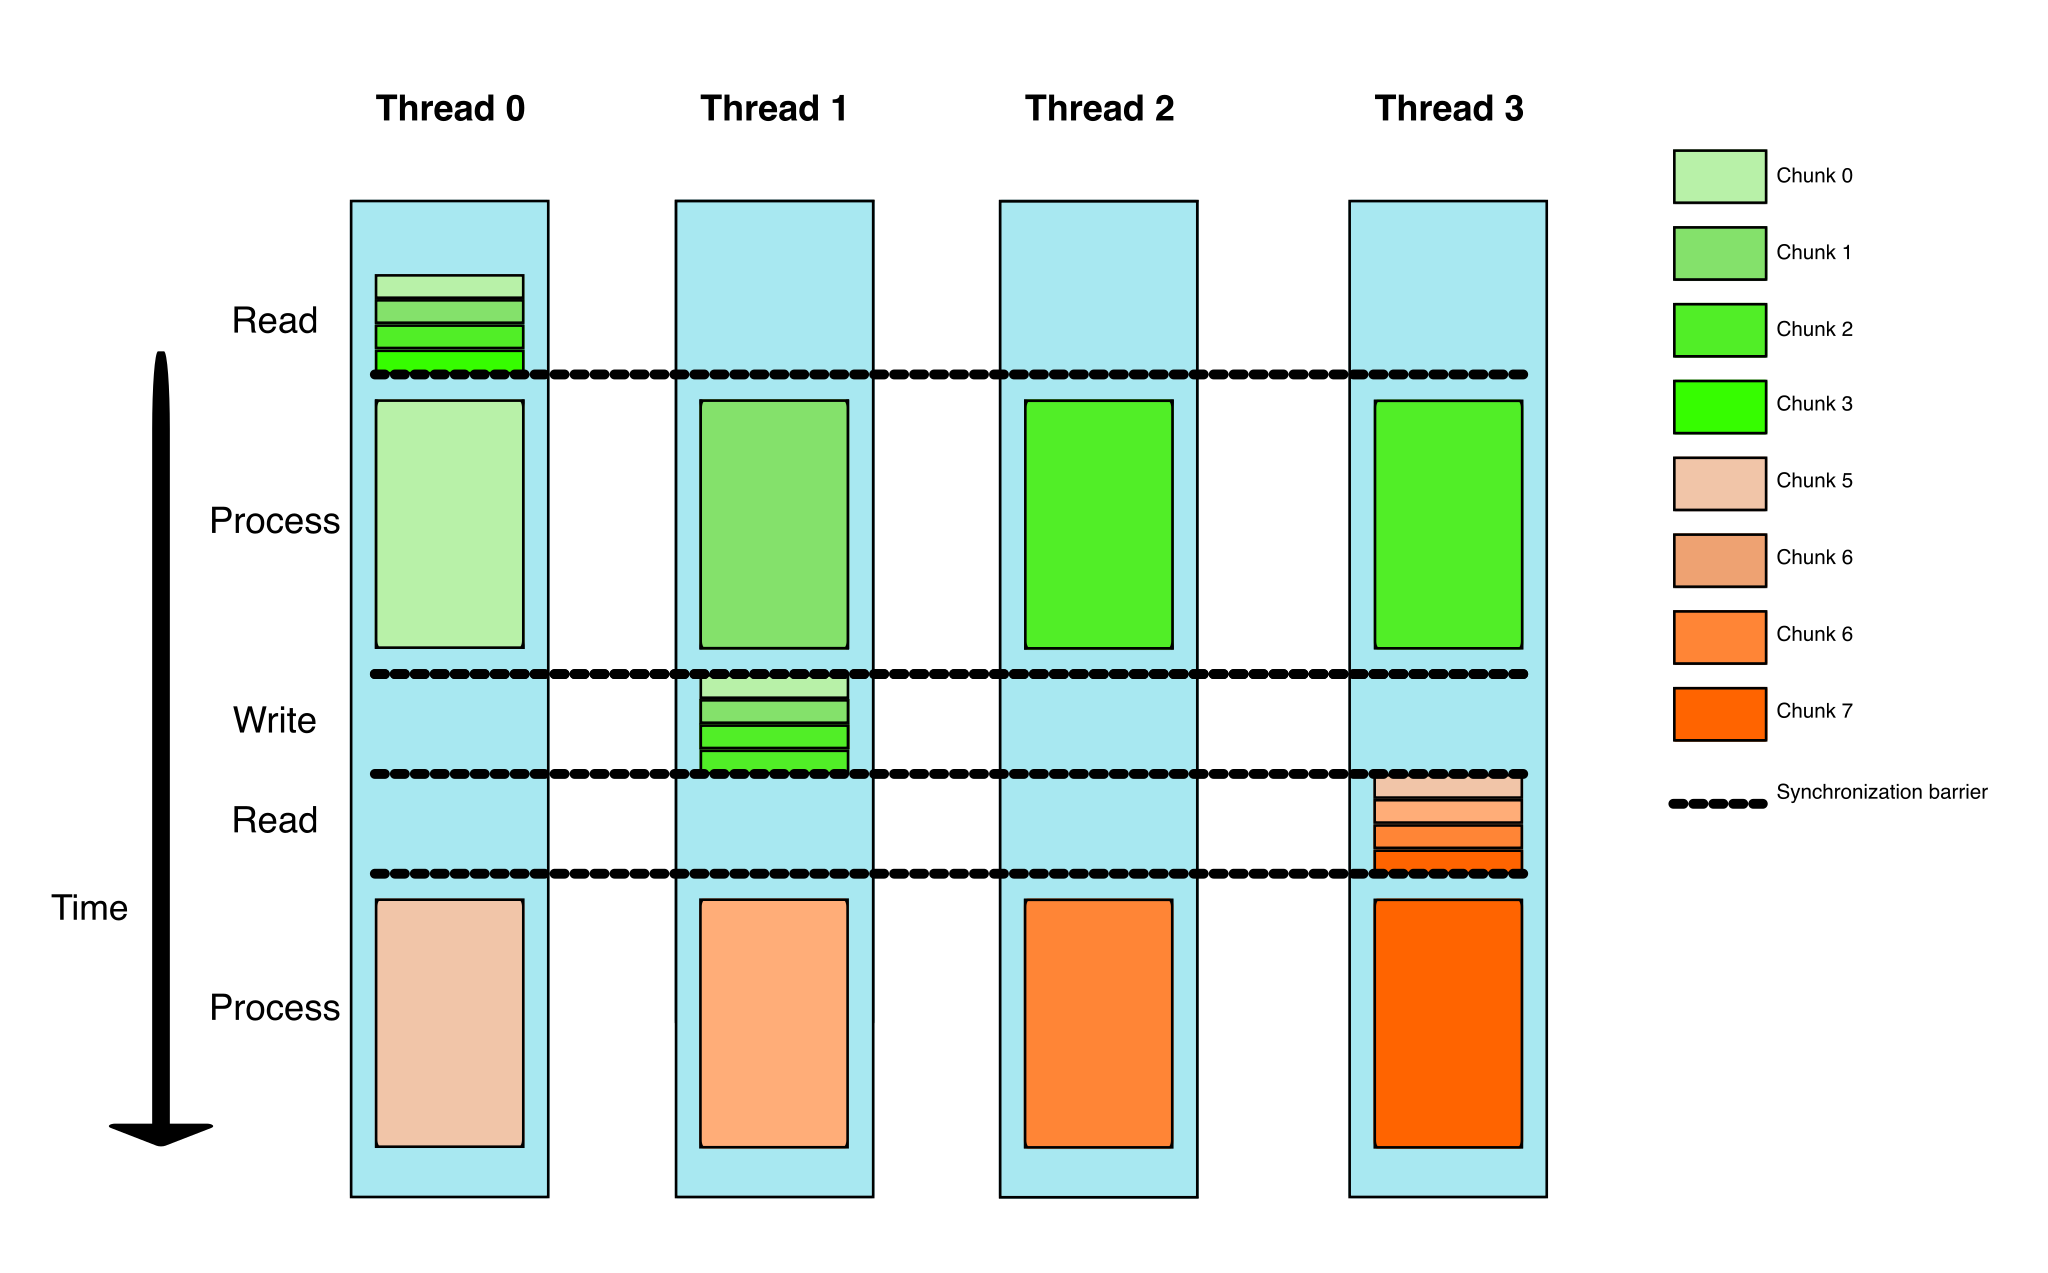
\includegraphics[width=0.8\linewidth]{../imgs/threading}
	\caption{Simple schema for processing a single file with multiple threads.}
	\label{fig:threading}
\end{figure}


\subsection{Multiprocessing}

Additionally, we wanted our tool to be able to process multiple files and folders: for this use case, we exploit multiprocessing.

To achieve this, we devised a simple algorithm to distribute files across multiple processes, so that each process can work on its own list of files, independently to others. In this way, we can minimize communication and therefore latency and other slowdowns between the different components of the applications. Suppose we are dealing with \(n\) process, \(m\) threads, and an input folder.

\begin{enumerate}
	\item First, the process with rank 0 (the main process) crawls all the files in the input directory recursively in all the subfolders.
	\item Then the rank 0 process opens all the files and reads their size.
	\item Once all files and their respective sizes are known, the main process creates a min priority queue where each item represents a process and its priority is the size of files that have been assigned to it.
	\item Process 0 can iteratively insert files in the priority queue and updates the priority of each process with the cumulative file size. The main idea is that we can ensure an equal work division among different processes.
	\item When all this is done, the main process sends the list of files to each process and then each starts to work independently on its own list of files.
\end{enumerate}

\subsection{Implementation details and other notes}
Here follows a list of further comments and design choices for our specific Huffman implementation. 

\begin{itemize}
\item We decided on an alphabet of 256 for the Huffman coding because this way we can encode each byte of the input data into a different Huffman code. As C language does not allow to address data at lower resolution than a byte, lowering the alphabet would not result in any perfomance benefit. We also considered encoding multiple bytes into a single huffman code, but that results in worse compression as the resulting huffman tree would have more leaves.

\item We found that a chunk size of 4096 bytes had the best I/O times. This is probably due to the fact that 4096 B is the size of a page in most Linux based operating systems. The last chunk of a file may be smaller. Reading any other size at the time had resulted in significantly worse I/O times (both increasing and decreasing the chunk size).

\item In general, all threads will finish processing their chunks at around the same time, but in some cases there are threads that can take longer. This is due to the very unlucky case where a whole chunk contains exclusively very infrequent bytes of data. Because the bytes are very infrequent, each one is encoded in extremely long sequences, up to 256 bits, resulting in a bigger encoded chunk than the original data. With our Huffman alphabet set to a single byte, the worst case results in having a compressed chunk being 32 times bigger than decompressed one.

\item We tried to parallelize the I/O, by having each thread read its own chunk. We found that the standard file descriptor provided by C have a lock to guarantee thread safety. Unfortunately, this lock slows down the reads significantly. We also tried using multiple file descriptors to circumvent this limitation, however we found no improvement over a single-thread sequential read. This is likely because the O.S. schedules I/O requests and serves them one at the time, resulting in an impossibility of having truly parallel I/O.

\item We also tested an architecture where we had two dedicated threads to I/O, one for reading and one for writing chunks. The idea is that whenever a chunk is processed, the I/O threads would immediately write the processed chunk to the output file and similarly a new chunk would be read from the input file (very similar to a queue of jobs). Theoretically this would allow to parallelize I/O and computation operations: in this scenario we avoided concurrency problems by synchronizing the I/O with locks. In later analysis we call this architecture "Locks" because of the synchronization method we are using.

\item Another detail we noticed on the implementation with two dedicated threads for I/O, is that if there are not enough cores on the CPU or if the operating system decides to allocate all the threads on a single processor, the encoding and decoding times are greatly affected by the scheduler. This is because it might be that the O.S. gives priority to threads that are waiting (for example the writer cannot write any block until the first has finished, even if all others have finished). In the worst case scenario, the multithreading architecture could be even slower that the serial one.

\end{itemize}
